
\begin{figure}
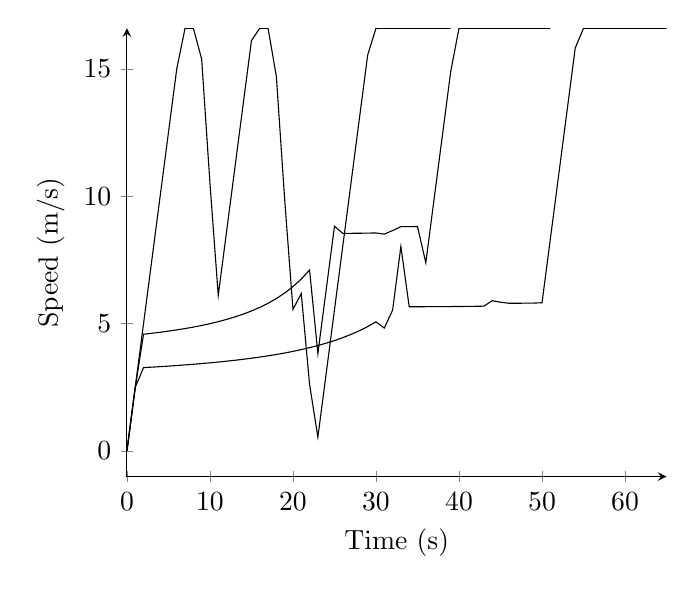
\begin{tikzpicture}
\begin{axis}[
legend style={
	anchor=west
},
axis x line=bottom,
axis y line=left,
ymin=-1,
point meta=explicit symbolic,
xlabel=Time (s),
ylabel=Speed (m/s)
]
\addplot[] coordinates {
(0, 0.0)
(1, 2.5)
(2, 4.58648543541)
(3, 4.623705462)
(4, 4.66416428807)
(5, 4.70825187145)
(6, 4.75641915816)
(7, 4.80918998811)
(8, 4.86717582304)
(9, 4.93109409275)
(10, 5.00179121866)
(11, 5.08027173788)
(12, 5.16773545915)
(13, 5.26562530211)
(14, 5.37568950269)
(15, 5.50006336659)
(16, 5.64137796398)
(17, 5.80290647328)
(18, 5.98876393866)
(19, 6.2041840689)
(20, 6.45590919037)
(21, 6.75274975203)
(22, 7.10640358635)
(23, 3.82855573542)
(24, 6.32855573542)
(25, 8.82855573542)
(26, 8.54592028659)
(27, 8.54848672963)
(28, 8.55185919229)
(29, 8.55641591492)
(30, 8.56278759713)
(31, 8.51802259135)
(32, 8.65764394997)
(33, 8.80979793751)
(34, 8.81158433644)
(35, 8.81564072674)
(36, 7.39233326267)
(37, 9.89233326267)
(38, 12.3923332627)
(39, 14.8923332627)
(40, 16.6)
(41, 16.6)
(42, 16.6)
(43, 16.6)
(44, 16.6)
(45, 16.6)
(46, 16.6)
(47, 16.6)
(48, 16.6)
(49, 16.6)
(50, 16.6)
(51, 16.6)
};
\addplot[] coordinates {
(0, 0.0)
(1, 2.5)
(2, 3.2760877681)
(3, 3.29479795165)
(4, 3.31464730346)
(5, 3.33573095234)
(6, 3.35815424946)
(7, 3.3820341258)
(8, 3.40750066608)
(9, 3.43469893993)
(10, 3.46379113971)
(11, 3.49495908544)
(12, 3.52840717126)
(13, 3.56436584513)
(14, 3.60309573569)
(15, 3.64489256848)
(16, 3.69009305001)
(17, 3.73908194508)
(18, 3.79230063379)
(19, 3.8502575151)
(20, 3.91354072922)
(21, 3.98283381275)
(22, 4.05893508986)
(23, 4.14278186011)
(24, 4.23548079627)
(25, 4.33834645296)
(26, 4.45295047017)
(27, 4.58118502264)
(28, 4.72534545374)
(29, 4.88823905042)
(30, 5.07332989478)
(31, 4.82892499961)
(32, 5.53100304923)
(33, 8.03100304923)
(34, 5.6657965551)
(35, 5.6667878924)
(36, 5.66796321467)
(37, 5.66937118492)
(38, 5.67107774958)
(39, 5.67317409812)
(40, 5.67578927603)
(41, 5.67911086199)
(42, 5.68342023727)
(43, 5.68915564417)
(44, 5.90287027895)
(45, 5.84347986935)
(46, 5.80314867249)
(47, 5.80423270644)
(48, 5.80617047414)
(49, 5.8102707345)
(50, 5.82270902365)
(51, 8.32270902365)
(52, 10.8227090236)
(53, 13.3227090236)
(54, 15.8227090236)
(55, 16.6)
(56, 16.6)
(57, 16.6)
(58, 16.6)
(59, 16.6)
(60, 16.6)
(61, 16.6)
(62, 16.6)
(63, 16.6)
(64, 16.6)
(65, 16.6)
};
\addplot[] coordinates {
(0, 0.0)
(1, 2.5)
(2, 5.0)
(3, 7.5)
(4, 10.0)
(5, 12.5)
(6, 15.0)
(7, 16.6)
(8, 16.6)
(9, 15.3934569437)
(10, 10.5214562517)
(11, 6.11202054391)
(12, 8.61202054391)
(13, 11.1120205439)
(14, 13.6120205439)
(15, 16.1120205439)
(16, 16.6)
(17, 16.6)
(18, 14.7050672306)
(19, 9.88203394578)
(20, 5.56090804849)
(21, 6.18702992217)
(22, 2.61854623807)
(23, 0.546509329476)
(24, 3.04650932948)
(25, 5.54650932948)
(26, 8.04650932948)
(27, 10.5465093295)
(28, 13.0465093295)
(29, 15.5465093295)
(30, 16.6)
(31, 16.6)
(32, 16.6)
(33, 16.6)
(34, 16.6)
(35, 16.6)
(36, 16.6)
(37, 16.6)
(38, 16.6)
(39, 16.6)
};

\end{axis}
\end{tikzpicture}
\label{tik:50:16_O, 17_S, 17_S.-60, 20_O, 21_O}
\caption{50 percent diving with GSC on route $16_O, 17_S, 17_S.-60, 20_O, 21_O$}
\end{figure}
